%!TEX encoding = UTF-8 Unicode
\documentclass{simpleslides}

%\usepackage{beamerthemesplit}
\usepackage[orientation=landscape,size=custom,width=10,height=9,scale=0.6,debug]{beamerposter} 

\definecolor{BG}{rgb}{0.88, 0.88, 0.95}%{gray}{0.88}
\setbeamercolor{background canvas}{bg=BG}

%\title[Föreläsning, EDAA45 pgk, Björn Regnell, senast uppdaterad: \today]{Vecka \vecka. \veckotema}
%\subtitle{Programmering, grundkurs}
\title{God digitalisering? \\ {\fontsize{10}{12}\selectfont Kravhantering \& öppenkällkod för en bättre värld}}
\author{Björn Regnell}
\institute{Professor i programvarusystem\\Datavetenskap, LTH, Lunds universitet}
%\date{EDAA45, Lp1-2, HT \CurrentYear}
\date{}

\setbeamersize{text margin left=18pt,text margin right=12pt}
\begin{document}
\settowidth{\leftmargini}{\usebeamertemplate{itemize item}}
\addtolength{\leftmargini}{-0\labelsep}


\frame{\titlepage}
%\setnextsection{\vecka}


%\frame{\tableofcontents}

%\section{God digitalisering?}


\begin{Slide}{Tekniksprång}
\begin{itemize}
  \item Domesticering  \hfill 10000 år sedan
  \item Mekanisering \hfill 500 år sedan
  \item Elektrifiering \hfill 250 år sedan
  \item Datorisering \hfill 50 år sedan
  \item Digitalisering \hfill 25 år sedan
  % \hfill
  % \begin{itemize}
  %   \item[] -- hela samhällets omvandlas från analogt till digitalt
  %   \item[] -- sammanvävda IT-system i nästan alla verksamheter
  %   \item[] -- sensorer och mjukvara nästan överallt
  % \end{itemize}
\end{itemize}
%~\\Digitalisering = genomgripande omvandling med informationsteknik
\end{Slide}


\newcommand{\Img}[3]{
{  \setbeamercolor{background canvas}{bg=black}
  \frame[plain]{\hspace*{#1}\includegraphics[height=#2\textheight]{#3}}
}}

\Img{-2.1cm}{1.05}{img/eniac}
\Img{-1.5cm}{1.1}{img/servers}
\Img{-1.2cm}{1.05}{img/ar}


\Subsection{Att skapa gemensam kunskap om framtiden}


\begin{Slide}{Systemutveckling}
\large  krav $\Rightarrow$ implementation $\Rightarrow$ drift \\~
\end{Slide}

\begin{Slide}{Systemutveckling}
\large  krav $\Leftrightarrow$ implementation $\Leftrightarrow$ drift \\ 
{ \vspace*{0.5em}\hspace*{0.8cm}\centering $\circlearrowright$ kontinuerlig leverans }
\end{Slide}



\begin{Slide}{\fontsize{20}{12}\selectfont Kravhantering =\\kollektivt kunskapsbyggande}
\begin{itemize}
\item Det räcker inte att kunna koda... 
\pause
\item Vi måste också tänka ut \Emph{vad} vi vill koda och avgöra om det är \Alert{rimligt} och \Alert{bra} att koda det vi vill!
\pause 
\item Vi skapar kunskap om framtidens system medan vi bygger dem.
\item Många kompetenser behövs: vi bygger vidare på varandras kunskaper.
\end{itemize}
\end{Slide}

\Subsection{{\small Valfri kurs i årskurs 4:}\\Kravhantering 7,5p\\{\small\texttt{https://cs.lth.se/krav}}}


\begin{Slide}{Vad behöver vi göra?}
% \begin{itemize}
% \item 
Kravhanteringens \Emph{sammanvävda} \textbf{grunduppgifter} pågår \Alert{ständigt}: \\~
\begin{itemize}
\item Elicitering \hfill lära
\item Specificering  \hfill modellera
\item Validering \hfill kolla
\item Selektering \hfill besluta
\end{itemize}
% \item
% När år vi färdiga?
%\end{itemize}
\end{Slide}

\begin{Slide}{Vad behöver vi kunskap om?}
Kravhanteringens \Emph{sammanvävda} \textbf{kunskapsområden} utvecklas \Alert{ständigt}: \\~
\begin{itemize}
\item Kontext \hfill vem
\item Intentioner  \hfill varför
\item Krav \hfill vad
\item Leverans \hfill när
\end{itemize}
\end{Slide}


\begin{Slide}{Hur ser sammanhanget ut?}
Den \Emph{komplexa} \textbf{kontexten} utvecklas \Alert{ständigt}: \\~
\begin{itemize}
\item Intressenter \hfill användare, makthavare
\item Vår produkt  \hfill avgränsning
\item Andra system \hfill samverkan
\item Gränssnitt \hfill interaktion, protokoll
\end{itemize}
\end{Slide}


\begin{Slide}{Vilka är våra intentioner?}
Olika \Emph{sammanvävda} \textbf{förutsättningar} utvecklas \Alert{ständigt}: \\~
\begin{itemize}
\item Mål \hfill intressebalans
\item Prioriteter  \hfill urval
\item Risker \hfill skada
\item Åtagande \hfill resurser
\end{itemize}
\end{Slide}

\begin{Slide}{Vilka typer av krav behövs?}
Olika \Emph{sammanvävda} \textbf{kravmodeller} utvecklas \Alert{ständigt}: \\~
\begin{itemize}
\item Funktionalitet \hfill effekt
\item Data  \hfill tillstånd
\item Kvalitet \hfill nytta
\item Testfall \hfill mätbara kriterier
\end{itemize}
\end{Slide}


\begin{Slide}{När leverera resultat?}
\Emph{Stegvisa} \textbf{resultat} levereras \Alert{kontinuerligt}: \\~
\begin{itemize}
\item Road-map \hfill strategi
\item Resurser  \hfill mänskliga, monetära
\item Begränsningar \hfill realism, villkor
\item Releaser \hfill tid, rum
\end{itemize}
\end{Slide}


\begin{Slide}{En checklista för ditt projekt:}
\hspace*{-0.55cm}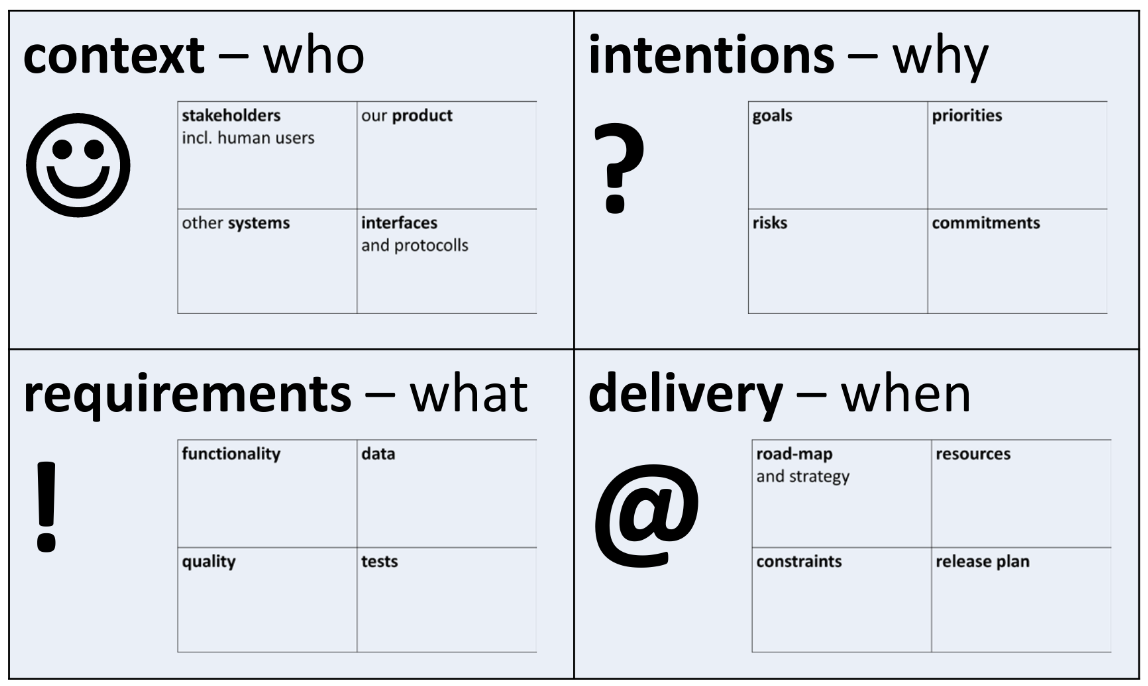
\includegraphics[width=1.1\textwidth]{img/reqt-box}

{\noindent\tiny\href{https://github.com/lunduniversity/reqeng/blob/master/reqtbox/reqtbox.pdf}{https://github.com/lunduniversity/reqeng/blob/master/reqtbox/reqtbox.pdf}}
\end{Slide}

\Subsection{Gemensam kunskap som öppen källkod}

%\Img{-0.7cm}{0.85}{img/earth-tree}

{  \setbeamercolor{background canvas}{bg=black}
\begin{Slide}{}
  \vspace*{-1.0cm}\hspace*{-0.75cm}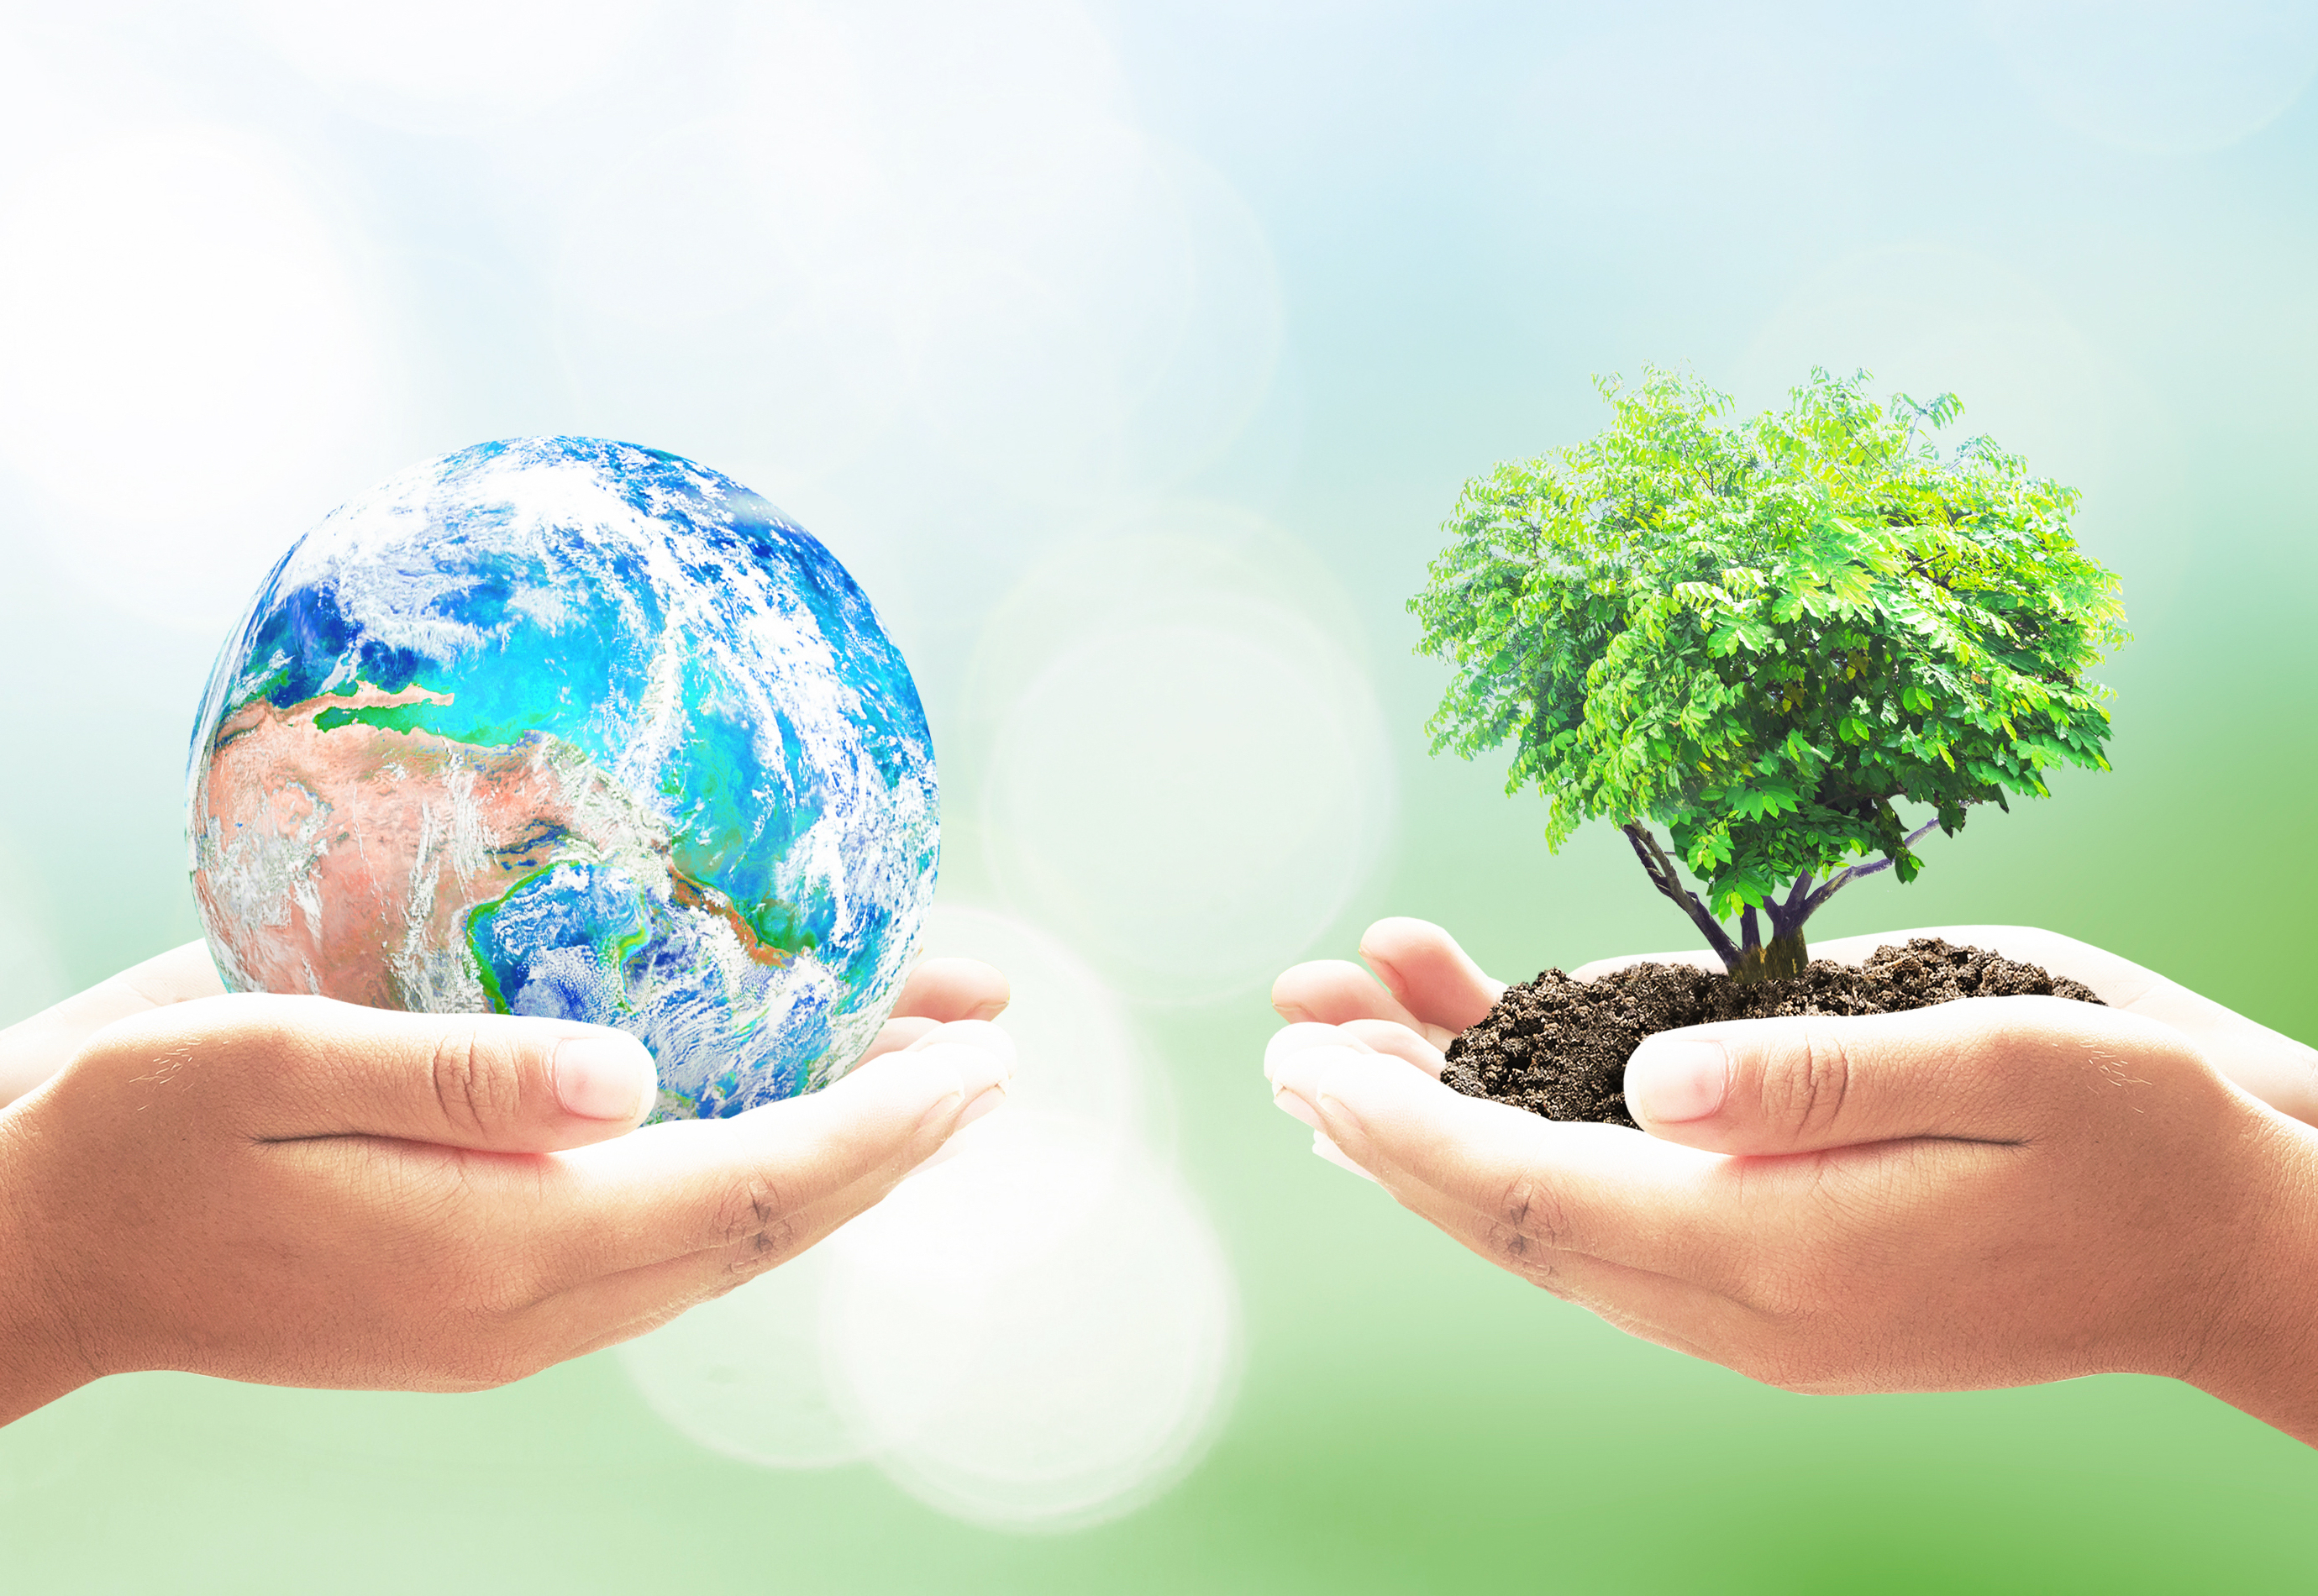
\includegraphics[width=1.2\textwidth]{img/earth-tree.jpg}

 {\fontsize{13}{13}\selectfont \Emph{Öppen källkod = våra digitala allmänningar}}
\end{Slide}
}

\begin{Slide}{Vad är öppen källkod?}
  \begin{itemize}
    \item  
  \end{itemize}
\end{Slide}


\Subsection{\texttt{cs.lth.se/krav}}  

\end{document}